\begin{frame}{Quels verbes?}
  La chanson suivante par Patrick Bruel s'appelle \href{https://youtu.be/Rglh1je-CrE?si=tLyIEmDT2dIacOfN}{Pour la vie}.
  À mesure que nous l'écoutons, notez tous les verbes pronominaux que vous entendez.
  \begin{columns}
    \column{0.5\textwidth}
      \begin{center}
        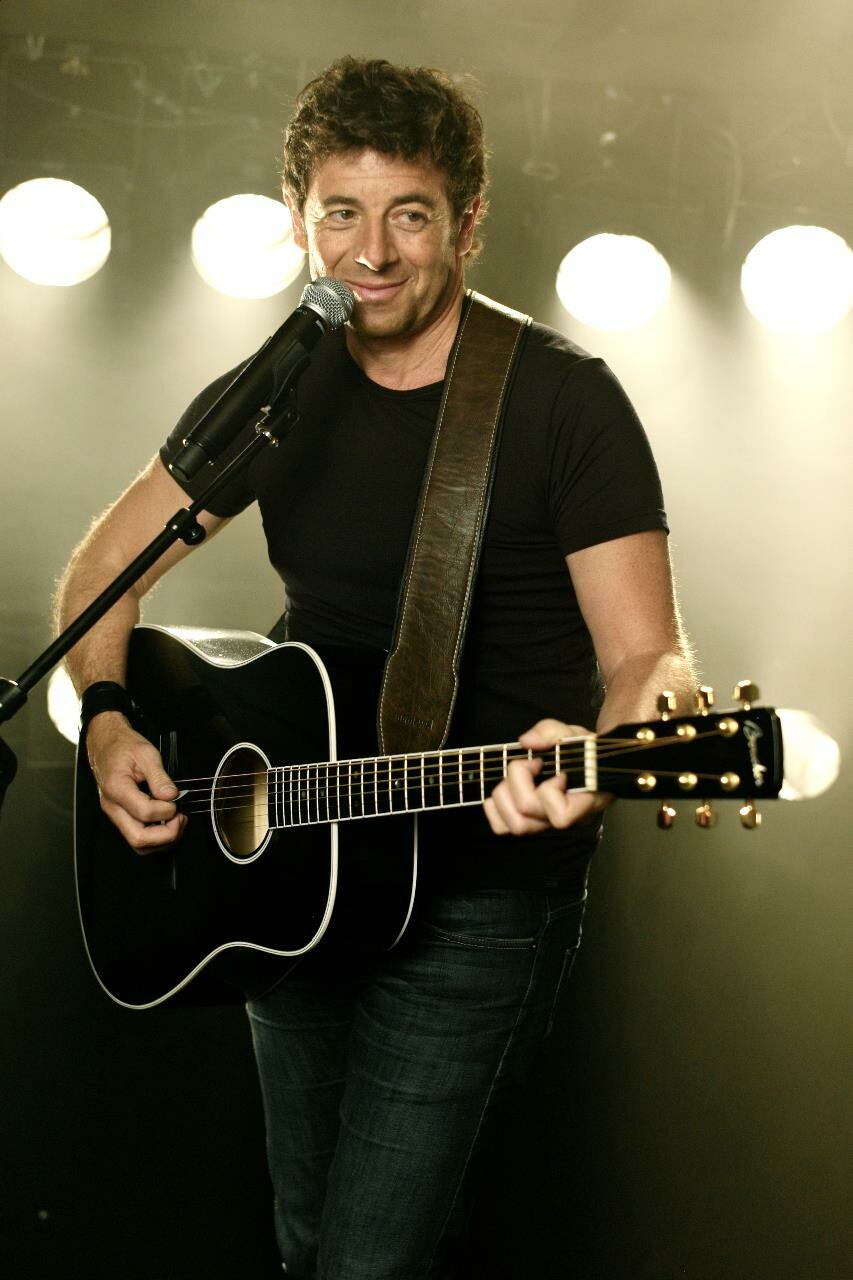
\includegraphics[scale=0.125]{patrick_bruel.jpg}
      \end{center}
    \column{0.5\textwidth}
      \uncover<2->{
        Les verbes:
        \begin{enumerate}
          \item s'embrasser
          \item se jurer
          \item se revoir
          \item s'inviter
          \item s'éviter
          \item se dire
          \item se souvenir
          \item se rappeler
        \end{enumerate}
      }
  \end{columns}
\end{frame}